\chapter{Qualitative Analysis with Rating Datasets Visualization}
\graphicspath{{Chapter06/Figures/}}
\label{chap:rs-viz}

Being able to correctly interpreting the results obtained during an offline evaluation of different recommender systems is of paramount importance for understanding the quality of the suggested items~\cite{Ge2010}. However, this task is particularly difficult as it requires knowing several details regarding the evaluation protocol~\cite{Said2014}. For this reason, in Chapter~\ref{chap:sequeval} and~\ref{chap:reclab}, we have formalized two evaluation frameworks to address the problem of reproducibility in recommender systems research.

In the following, we consider the task of characterizing the rating dataset exploited for conducting the experiments, as it has a profound impact on the final result. For example, sparse datasets usually yield to lower evaluation scores with respect to more dense datasets~\cite{Cremonesi2010}. On the other hand, datasets with many popular items tend to advantage systems that create less diverse suggestions~\cite{Vargas2011}, like the most popular baseline. There are also some subtle differences among rating datasets related to the application domain or the collection protocol that could affect the choice of the most appropriate recommender system.

Different metrics have been proposed in literature to summarize the main characteristic of a rating dataset, i.e. sparsity or entropy. However, we argue that such metrics are not sufficient for comparing datasets in a reliable way, as many other facets should be taken into account. For example, it is not possible to understand the rating behaviors of specific groups of users nor the popularity of the most rated items by only looking at some general statistics computed on the whole dataset.

A possible solution to this problem could be represented by data visualization techniques~\cite{Kunkel2017}. However, most of the methods available in literature are designed to display the output of a recommendation model and not the original dataset~\cite{Gil2018,Cardoso2019}. In contrast, we argue that it is necessary to visually explore a rating dataset even before it is used to train a recommender system, for understanding how the input data will influence the outputs under analysis.

In this chapter, we propose a novel qualitative approach based on data visualization for creating a graphical summary of any collection of user preferences. This method is useful for visually identifying similarities and differences among the available datasets. In fact, we argue that if two datasets result in similar visualizations, the behavior of different recommender systems relying on them will be consistent. Furthermore, we present a Web-based tool, named RS-viz, for easily constructing the proposed visualization and comparing rating datasets in an intuitive way. The software code of RS-viz is freely available on GitHub.\footnote{\url{https://github.com/D2KLab/rs-viz}}

Differently from the plotting capabilities already available in specialized software like Matlab or Scilab, our approach is more general, as it can be applied in a consistent way by different users on any dataset and it can be exploited on many devices without the need of installing specific tools.

The remainder of this chapter is structured as follows: in Section~\ref{viz:sec:visualization} we present the approach used to construct the scatter plot and we describe the implementation details of the Web-based tool RS-viz. In Section~\ref{viz:sec:evaluation}, we comment on the outcome of an evaluation campaign designed to validate the proposed method. Finally, in Section~\ref{viz:sec:conclusion}, we provide the conclusions.

\section{Visualization Approach}
\label{viz:sec:visualization}

In this section, we first describe the algorithm that we devised for creating a scatter plot that represents a rating dataset (Section~\ref{viz:sec:scatter}), then we introduce the implementation details of RS-viz (Section~\ref{viz:sec:implementation}).

\subsection{Scatter Plot Construction}
\label{viz:sec:scatter}

For visually representing the rating matrix associated with a generic dataset we opted for a 3D scatter plot. The rationale behind this choice is that each point in the visualization could intuitively represent a single rating from the dataset: the value of the \textit{x}-axis is the identifier of the user, the value of the \textit{y}-axis is the identifier of the item, while the value of the \textit{z}-axis is the rating itself, if it is expressed on a numerical scale.

However, it is easy to foresee that this approach cannot handle complex datasets with many preferences, as it requires one point for each rating. If the ratings available are only binary, a traditional scatter plot would suffice.

For these reasons, we decided to create a more compact representation of the rating matrix before visualizing it. In details, we first associated the users and the items with internal numerical identifiers according to their frequency of appearance in the dataset. Therefore, we associated the most rated item with the value of~$1$, and the second most rated item with the value of $2$. The same approach was followed for ordering the identifiers of the users according to the number of ratings that they expressed.

Then, we linearly normalized such identifiers within an interval ranging from~$0$ to a user provided value, which represents the size of a squared rating matrix in a transformed space. Finally, we binarized the ratings from the original dataset according to a user provided threshold and we counted, for each cell of the transformed matrix, the number of positive preferences associated with that cell.

For example, if the user $40$ expressed a preference for the item $360$ in a dataset where the number of users is $941$, the number of items is $1446$, and the number of normalized users and items is equal to $100$, that rating would be associated with the cell $(4, 24)$ because $\lfloor 40 \div 941 \times 100 \rfloor = 4$ and $\lfloor 360 \div 1446 \times 100 \rfloor = 24$.

Therefore, the value of the \textit{z}-axis represents the number of positive ratings associated with a sub-matrix of the original dataset, sorted by item popularity and user activity. In order to enhance the readability of the visualization, we also represented the value of the \textit{z}-axis using a logarithmic color scale.

As an example of the proposed method, we report in Figure~\ref{viz:fig:ml-100k} and Figure~\ref{viz:fig:ml-1m} the scatter plots obtained from the MovieLens~100K and MovieLens~1M datasets, when the rating threshold is equal to~$3$, and the number of normalized users and items is equal to $100$.

By looking at the values of the \textit{z}-axis, it is possible to observe in an intuitive way that MovieLens~1M contains a higher number of popular items and of very active users. This conclusion is consistent with the findings of other works that analyze the main characteristics of the MovieLens datasets~\cite{Cremonesi2010}.

\begin{figure}
\centering
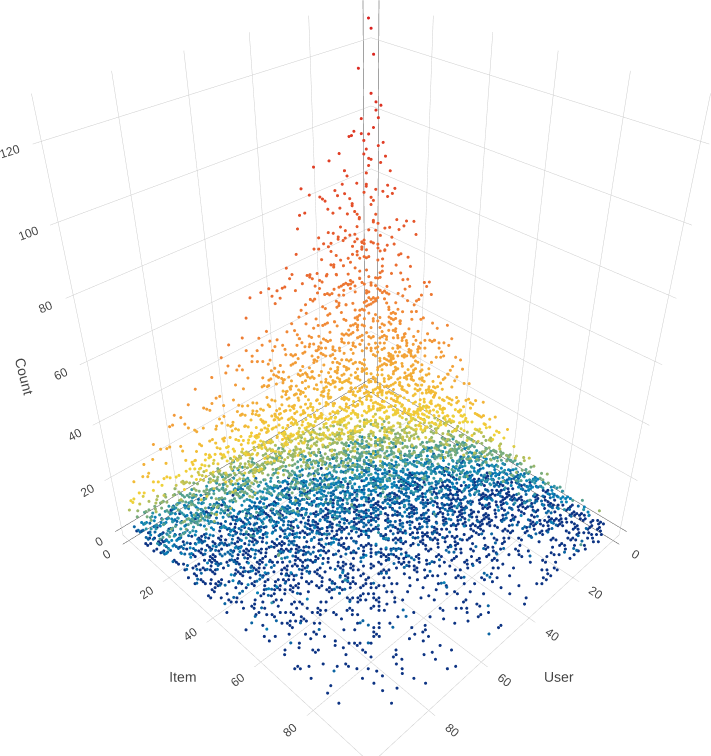
\includegraphics[width=.75\textwidth]{ml-100k}
\caption[Scatter plot of MovieLens~100K]{A scatter plot representing the MovieLens~100K dataset.}
\label{viz:fig:ml-100k}
\end{figure}

\begin{figure}
\centering
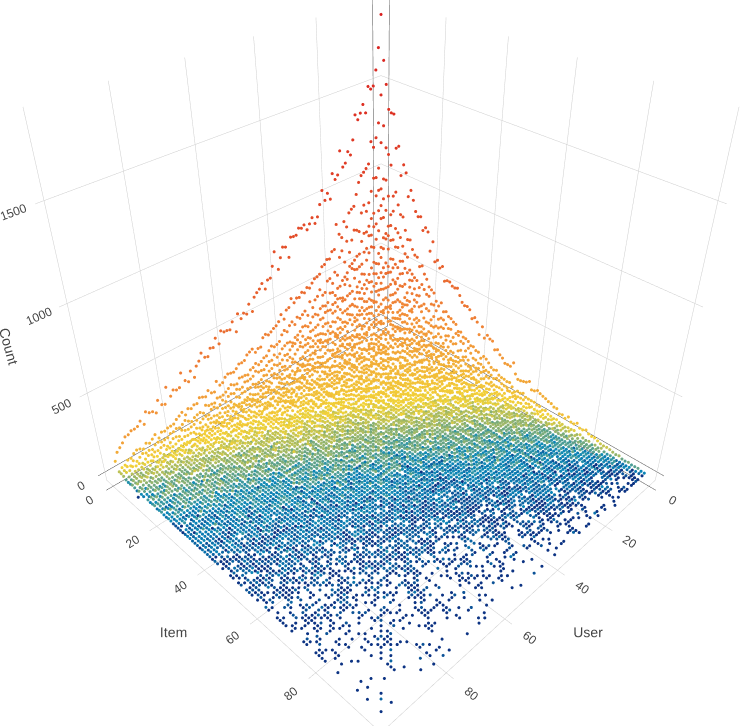
\includegraphics[width=.75\textwidth]{ml-1m}
\caption[Scatter plot of MovieLens~1M]{A scatter plot representing the MovieLens~1M dataset.}
\label{viz:fig:ml-1m}
\end{figure}

\subsection{Software Implementation}
\label{viz:sec:implementation}

We realized a software implementation of the proposed approach as a Web-based tool, called RS-viz, which is freely available. Our visualization framework has been developed using the JavaScript programming language and it runs entirely in a user's browser. For this reason, it can also be exploited for analyzing private datasets, as no information about them is sent to remote servers.

The user needs to visit the Web-page of RS-viz\footnote{\url{https://d2klab.github.io/rs-viz/}} and select one of the built-in datasets or provide her own dataset as a CSV file. Then, she needs to specify the threshold between positive and negative ratings and the number of normalized users and items, which should be selected also considering the rating scale of the input dataset and the desired visualization density. A screenshot of the form containing the configuration parameters of RS-viz is reported in Figure~\ref{viz:fig:rs-viz}.

After a few seconds, an interactive 3D scatter plot is constructed on the right side of the page. The user can inspect the plot by rotating the camera and finally save the result as a PNG file.

\begin{figure}
\centering
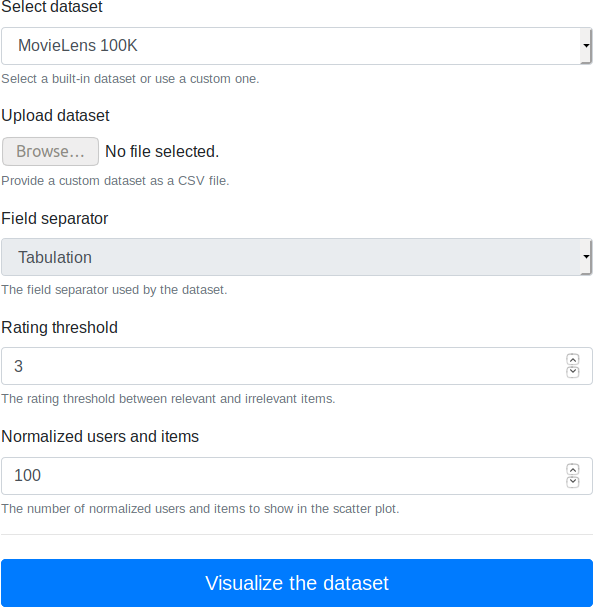
\includegraphics[width=.75\textwidth]{rs-viz}
\caption[Configuration of RS-viz]{The configuration parameters of RS-viz.}
\label{viz:fig:rs-viz}
\end{figure}

\section{Evaluation Campaign}
\label{viz:sec:evaluation}

In the following, we report the numerical outcomes of an evaluation campaign conducted on the HetRec LastFM dataset using different recommendation approaches with the purpose of understanding if our visualization technique is capable of capturing the different characteristics of a rating dataset and to what extend they influence the recommendation coverage and accuracy.

\subsection{Experimental Setup}

We performed two different experiments with the HetRec LastFM dataset and our evaluation framework RecLab, discussed in Chapter~\ref{chap:reclab}.

In the first one, we set the rating threshold equal to 0, while in the second one, we set it equal to 1,000. For the other parameters, we used the default values of the framework: we selected a random splitting protocol, the test set size as the 20\% of the dataset, and the length $k$ of the recommended lists equal to $10$.

We considered different recommendation approaches, namely the most popular and random baselines and the MyMediaLite~\cite{Gantner2011} implementations of the Item KNN, User KNN, BPRMF, and WRMF recommender systems using their default settings.

We computed the metrics of coverage, precision, recall, and NDCG. The results of these experiments are reported in Table~\ref{viz:tab:experiment}. The same datasets obtained from HetRec LastFM by varying the rating threshold were exploited for creating two scatter plots using RS-viz, as displayed in Figure~\ref{viz:fig:lastfm}.

\begin{table}
\begin{subfigure}{\textwidth}
\centering
\begin{tabular}{@{}lllll@{}}
\toprule
Algorithm & Coverage & Precision & Recall & NDCG \\ \midrule
Random & 0.706679 & 0.000798 & 0.000745 & 0.000858 \\
Most Popular & 0.001692 & 0.071170 & 0.071480 & 0.079673 \\
Item KNN & 0.235321 & 0.129362 & 0.131967 & 0.145258 \\
User KNN & 0.030074 & 0.157234 & 0.160353 & 0.193121 \\
BPRMF & 0.022979 & 0.081277 & 0.082248 & 0.094737 \\
WRMF & 0.015558 & 0.159947 & 0.162332 & 0.195107 \\ \bottomrule
\end{tabular}
\caption{Rating threshold = 0}
\bigskip
\end{subfigure}
\begin{subfigure}{\textwidth}
\centering
\begin{tabular}{@{}lllll@{}}
\toprule
Algorithm & Coverage & Precision & Recall & NDCG \\ \midrule
Random & 0.705562 & 0.000107 & 0.000622 & 0.000133 \\
Most Popular & 0.001684 & 0.022122 & 0.090233 & 0.027437 \\
Item KNN & 0.107233 & 0.002878 & 0.013012 & 0.002686 \\
User KNN & 0.049343 & 0.040672 & 0.160767 & 0.055013 \\
BPRMF & 0.003756 & 0.021695 & 0.088211 & 0.024366 \\
WRMF & 0.012886 & 0.039606 & 0.157484 & 0.053148 \\ \bottomrule
\end{tabular}
\caption{Rating threshold = 1,000}
\end{subfigure}
\caption[Experimental comparison with LastFM]{The numerical results of the experimental comparison using the HetRec LastFM dataset.}
\label{viz:tab:experiment}
\end{table}

\begin{figure}
\centering
\begin{subfigure}{.63\textwidth}
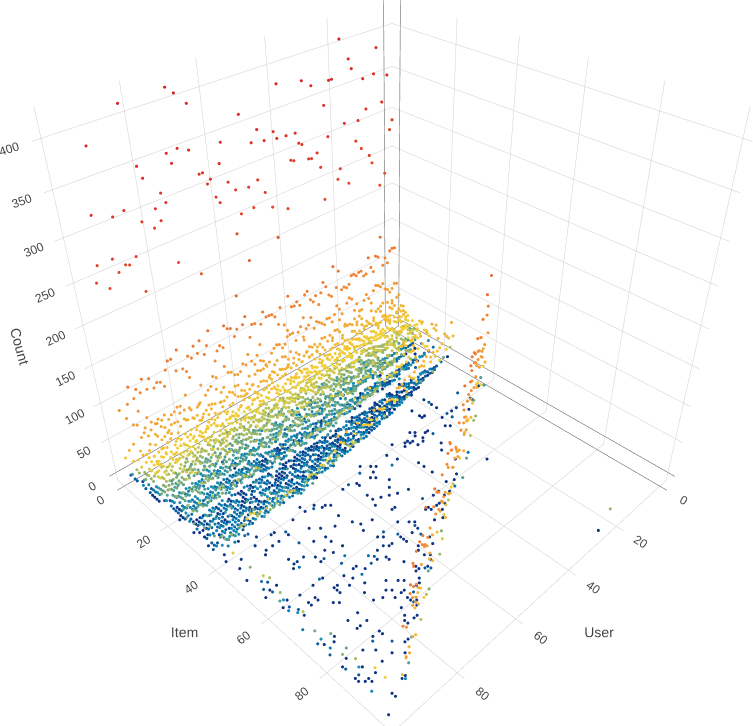
\includegraphics[width=\textwidth]{lastfm-t0}
\caption{Rating threshold = 0}
\label{viz:fig:lastfm-t0}
\bigskip
\end{subfigure}
\begin{subfigure}{.63\textwidth}
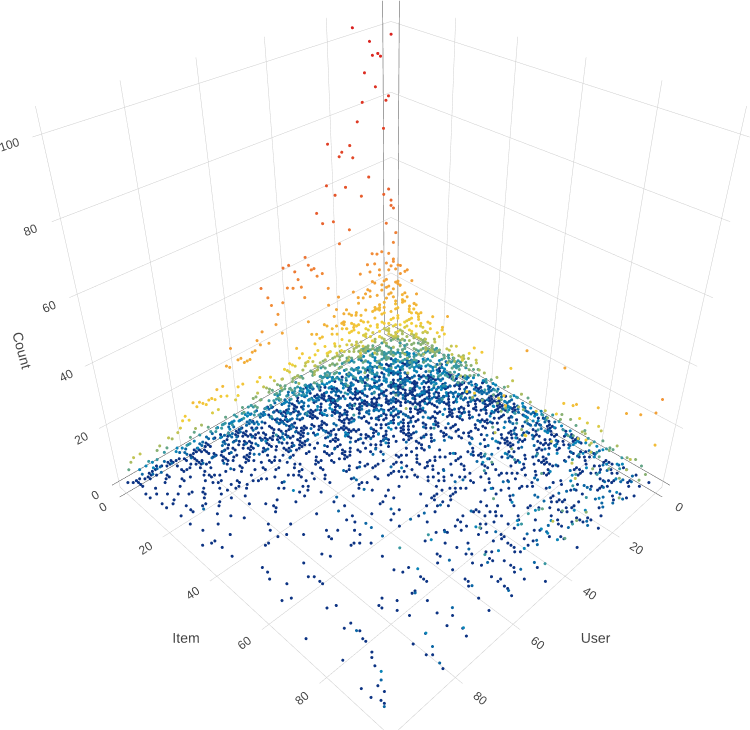
\includegraphics[width=\textwidth]{lastfm-t1k}
\caption{Rating threshold = 1,000}
\label{viz:fig:lastfm-t1k}
\end{subfigure}
\caption[Scatter plots of LastFM]{The scatter plots obtained using the HetRec LastFM dataset with different rating thresholds.}
\label{viz:fig:lastfm}
\end{figure}

\subsection{Discussion}

From the visualization provided in Figure~\ref{viz:fig:lastfm-t0}, we can observe that the HetRec LastFM dataset has a very different structure from the one of the MovieLens datasets. In fact, a limited number of items are associated with the preferences of almost all users, as it can be deduced by considering only the ratings expressed for popular items, that is the ones with low identifiers. Please note that such ratings seem not related to the identifier of the user, resulting in a scatter plot that resembles the shape of a half cylinder.

Furthermore, less popular items seem to be liked by less active users. This behavior can be observed by looking at the lower part of Figure~\ref{viz:fig:lastfm-t0}. Users with a high identifier have rated a more widespread set of items, while users with a low identifier have rated popular items more frequently.

These differences can be easily explained if we consider the collection protocol and the domain of the dataset under analysis. The ratings in the LastFM datasets represent the number of times a user listened to a particular artist: they were collected in an implicit way and their values range from one to tens of thousands.

Also the strange area in the plot with almost no preferences is a direct result of the collection protocol, which relied on the LastFM website to obtain the top artists for a set of users. In fact, the list of artists available in the dataset is limited to $50$ items for each user.

If we increase the value of the rating threshold, we can observe that the resulting scatter plot represented in Figure~\ref{viz:fig:lastfm-t1k} is more similar to the ones of the MovieLens datasets, resulting in a very typical long tail distribution with respect to both the items and the users. This outcome is due to the fact that we removed ratings produced by more casual listeners.

From the numerical outcomes of the experiments, we can deduce that the User KNN and WRMF algorithms are the most appropriate ones with both the different rating thresholds. In general, all the recommenders available perform worse with an higher threshold. In fact, from the visualizations it is clear that the number of available preferences is much lower with respect to the MovieLens~100K dataset, as the scatter plot represented in Figure~\ref{viz:fig:lastfm-t1k} is sparser than the one available in Figure~\ref{viz:fig:ml-100k}. Because user preferences are more limited in number and fragmented, the task of any recommender system is necessarily harder.

Interestingly, the Item KNN, differently from the User KNN, experienced a dramatic drop in all the metrics considered. This result may have been caused by the fact that a very low number of users is available for each item of the dataset. Also this characteristic can be observed from the generated scatter plot by looking at the lower part of Figure~\ref{viz:fig:lastfm-t1k}. The white horizontal stripes denote groups of items that have been rated by only a few very active users.

\section{Conclusion}
\label{viz:sec:conclusion}

In this chapter, we proposed a method for creating graphical summaries of any rating dataset for the purpose of enabling researchers and practitioners to better interpret the results of an offline evaluation campaign. Furthermore, we introduced RS-viz, a Web-based tool capable of creating an interactive 3D scatter plot according to the aforementioned approach starting from a user provided CSV dataset or a built-in collection of ratings.

We validated the capabilities of such visualizations to reveal useful information by comparing the graphical representations of the HetRec LastFM dataset constructed with different rating thresholds with the numerical outcomes of two offline experiments involving various recommendation techniques.
